\chapter{Manifolds}
\section{Definition}
The basic idea is that a manifold is an object $M$ that looks locally like a piece of $\R^n$, i.e. around any point we can find an area small enough that it looks flat.
\begin{definition}
A topological space $M$ is \udef{locally Euclidean} of dimension $n$ is every point $p\in M$ has a neighbourhood $U$ such that there is a homeomorphism $\phi$ from $U$ onto an open subset of $\R^n$. We call
\begin{itemize}
\item the pair $(U,\phi:U\to \R^n)$ a \udef{chart};
\item $U$ a \udef{coordinate neighbourhood} or a \udef{coordinate open set};
\item $\phi$ a \udef{coordinate map} or a \udef{coordinate system} on $U$:
\[ \phi:U\to \R^n: p\mapsto (x^1(p), \ldots, x^n(p)). \]
\end{itemize}
A chart $(U,\phi)$ is \udef{centred at} $p\in U$ if $\phi(p) = \vec{0}$. A \udef{chart about} $p$ is a chart $(U,\phi)$ such that $p\in U$.
\end{definition}
TODO: for well defined: open subsets of $\R^m$ and $\R^n$ cannot be homeomorphic if $n\neq m$.
\begin{definition}
An $n$-dimensional \udef{(topological) manifold} $M$ is a second-countable, Hausdorff topological space that is locally Euclidean of dimension $n$.
\end{definition}
[Picture with manifold and overlapping patches mapping to Rm phi1 phi2 + mappings between R's .]

By requiring the topology to be second-countable (C2) and Hausdorff, we immediately guaranty our manifold has whole load of nice properties. An important one is the ability to embed manifolds in higher-dimensional Euclidean spaces (cfr. Whitney's embedding theorem). Other properties that second-countable Hausdorff spaces have include being metrizable, completely normal and paracompact.

Also note that subspaces of a Hausdorff (resp. C2) space are automatically Hausdorff (resp. C2).

\begin{proposition}
Every discrete space is a $0$-dimensional manifold.
\end{proposition}
\begin{lemma}
Every manifold is locally path-connected.
\end{lemma}
This follows from the homeomorphisms with the path-connected space $\R^n$. Thus for manifolds the notions of connectedness and path-connectedness coincide.

\begin{definition}
Let $(U,\phi), (V,\psi)$ be two charts such that $U\cap V \neq \emptyset$. The maps
\[ \phi\circ\psi^{-1}:\psi(U\cap V)\to \phi(U\cap V) \qquad \text{and} \qquad \psi\circ\phi^{-1}:\phi(U\cap V)\to \psi(U\cap V) \]
are called \udef{transition functions} or \udef{change of coordinate maps}.
\end{definition}
Transition functions are compositions of homeomorphisms and thus homeomorphisms.

\begin{definition}
An \udef{atlas} on a manifold $M$ is a collection of charts $\{(U_\alpha, \phi_\alpha)\}$ that covers $M$, i.e. $M=\bigcup_\alpha U_\alpha$.
\end{definition}

\section{Types of manifolds}
Manifolds are very useful in many areas of physics and mathematics. Consequently there are many extensions and types of manifolds.
\subsection{Topological manifolds}
Topological manifolds are manifolds with no additional structure. The moniker topological is redundant, but can be used to emphasise that there is no additional structure, or, if there was previously additional structure, that one should forget about that additional structure.
\subsection{Differential manifolds} 
Differential manifolds have an atlas that allows differential calculus to be used on the manifold.

Each chart allows the use of calculus using the standard differential structure on linear space. (TODO!) The only difficulty is with the transition maps.
\begin{definition}
Two charts are called \udef{$C^k$-compatible} if the transition functions are in $C^k$.
\end{definition}

\begin{definition}
A $C^k$ \udef{atlas} on a manifold $M$ is a collection  $\{(U_\alpha, \phi_\alpha)\}$ of \udef{$C^k$-compatible} charts that covers $M$, i.e. $M=\bigcup_\alpha U_\alpha$.
\end{definition}

\begin{lemma}
Let $\{(U_\alpha, \phi_\alpha\}$ be an atlas. If two charts $(V,\psi)$ and $(W,\sigma)$ are compatible with the atlas, they are compatible with each other.
\end{lemma}

Two atlases are \udef{$C^k$-equivalent} if the union of their sets of charts forms a $C^k$-atlas.

\begin{lemma}
The $C^k$-equivalence of atlases is an equivalence relation. Each equivalence class is called a distinct \udef{$C^k$ differential structure} of the manifold.
\end{lemma}

A \udef{maximal atlas} is an atlas that is not contained in a larger atlas.

\begin{lemma}
The union of a $C^k$-equivalence class is a maximal atlas. Conversely every maximal atlas is the union of a $C^k$-equivalence class.
\end{lemma}
A differential structure is sometimes defined as a maximal atlas. By this lemma this is equivalent.

\begin{corollary}
Any atlas is contained in a unique maximal atlas.
\end{corollary}

\begin{definition}
A \udef{differential manifold} is a manifold with a $C^k$ differential structure.
\end{definition}
In fact we can even recover the manifold from the differential structure

It is however not meaningful to talk of a $C^k$-manifold as any manifold with a $C^k$-atlas with $k>0$ can be given a $C^\infty$-atlas. In fact every $C^k$-structure is uniquely \textit{smoothable} to a $C^\infty$-structure.

The differential structure allows the definition of the globally differentiable tangent space. This process is discussed in the next section.

A manifold may also be defined as an equivalence class of atlases (TODO).

In dimensions smaller than $4$ every topological manifold has a unique differentiable structure and in dimensions larger than $4$ every compact topological manifold hasa finite number of differentiable structures. Dimension 4 is a mystery.

There are topological manifolds with no differentiable structure.

\subsection{Smooth manifolds}
Smooth manifolds are differentiable manifolds for which all the transition maps are smooth (i.e. infinitely differentiable). All concepts in the previous section relating to differential manifolds apply if $C^k$ is replaced by $C^\infty$ or ``smooth''.

We will see later that:
\begin{proposition}
Every differential manifold is uniquely smoothable. I.e. every $C^k$ differential structure has a unique $C^\infty$ structure that is $C^k$ equivalent.
\end{proposition}
Consequently there is no real difference between differential and smooth manifolds. We will mainly study the latter.


\subsection{Analytic manifolds}
Analytic manifolds are smooth manifolds with the additional condition that each transition map is analytic or $C^\omega$: the Taylor expansion is absolutely convergent and equals the function on some open ball.

\section{Manifolds with boundaries}

\section{Submanifolds}




\chapter{Smooth manifolds}
In this chapter all manifolds are assumed smooth, i.e. $C^\infty$.
\section{The tangent space}
\subsection{Functions on manifolds}
\begin{definition}
Let $M,N$ be manifolds of dimension $m,n$. A map $F: M \to N$ is said to be \udef{smooth}, or $C^\infty$, at a point $p\in M$ if there are charts $(U,\phi)$ about $p\in M$ and $(V,\psi)$ about $F(p) \in N$ such that
\[ \psi \circ F \circ \phi^{-1}: \phi[F^{-1}[V]\cap U]\subset \R^m \to \R^n \]
is smooth at $\phi(p)$.

The function $F: M\to N$ is said to be \udef{smooth} if it is smooth are every point $p\in M$.
\end{definition}
Notice that the smoothness of a function is independent of the charts chosen:
\begin{lemma}
Let $M,N$ be manifolds of dimension $m,n$. If a function $F: M\to N$ is smooth at $p\in M$, then for any charts $(U',\phi')$ about $p\in M$ and $(V',\psi')$ about $F(p)\in N$,
\[ \psi'\circ F \circ (\phi')^{-1}: \phi'[F^{-1}[V']\cap U']\subset \R^m \to \R^n \]
is $C^\infty$ at $\phi'(p)$.
\end{lemma}
\begin{proof}
Let $F: M\to N$ be smooth and $p\in M$, $(U,\phi), (V,\psi)$ be as in the definition. Then
\[ \psi' F\circ (\phi')^{-1} = (\psi'\circ \psi)\circ(\psi F\circ \phi^{-1})\circ (\phi \circ (\phi')^{-1}) \]
is smooth at $\phi'(p)$, because it is a composition of smooth maps.
\end{proof}

\begin{lemma}
Let $F: M\to N$ and $G: N\to P$ be smooth maps of manifolds, then $G\circ F$ is smooth.
\end{lemma}

\begin{definition}
A \udef{diffeomorphism of manifolds} is a bijective $C^\infty$ maps $F:M\to N$ such that $F^{-1}$ is also $C^\infty$.
\end{definition}

\begin{lemma}
If $(U,\phi)$ is a chart on a manifold $M$, then the coordinate map $\phi$ is a diffeomorphism.
\end{lemma}
\begin{proof}
By definition $\phi: U \subset M \to \phi(U) \subset \R^n$ is a homeomorphism, so we just need to check $\phi$ and $\phi^{-1}$ are smooth.  Let $(\R^n, I_{\R^n})$ be a chart of $\R^n$. Then 
\[ I_{\R^n} \circ \phi \circ \phi^{-1} \qquad \text{and} \qquad \phi\circ \phi^{-1}\circ I_{\R^n} \]
are both the identity map and thus smooth, so both $\phi$ and $\phi^{-1}$ are $C^\infty$.
\end{proof}

\begin{lemma}
Let $U$ be an open subset of a manifold $M$ of dimension $n$. If $F: U\to \R^n$ is a diffeomorphism into an open subset of $\R^n$, the $(U,F)$ is a chart in the differentiable structure of $M$.
\end{lemma}


$C^\infty(M)$; $C^\infty(M)_p$ algebra of germs of functions in $C^\infty(M)$ at $p$.
TODO Pullback? Previous chapter?

\subsection{Derivatives of functions on manifolds}
Let $r^1,\ldots,r^n$ denote the standard coordinates on $\R^n$. Then $x^i = r^i\circ \phi$.
\begin{definition}
Let $p\in U$. We define the partial derivative $\pd{f}{{x^i}}$ at the point $p$ as
\[ \left.\pd{}{x^i}\right|_p f \defeq \pd{(f\circ\phi^{-1})}{r^i}(\phi(p)). \]
\end{definition}
Alternatively, as a function on $\phi(U)$, we write
\[ \pd{f}{x^i}\circ\phi^{-1} = \pd{(f\circ\phi^{-1})}{r^i}. \]

\begin{proposition}
Let $(U,(x^1,\ldots, x^n))$ be a chart on a manifold. Then
\[ \pd{x^i}{x^j} = \delta^i_j. \]
\end{proposition}
\begin{proof}
By direct computation:
\[ \pd{x^i}{x^j}(p) = \pd{(x^i\circ\phi^{-1})}{r^j}(\phi(p)) = \pd{(r^i\circ \phi\circ\phi^{-1})}{r^j}(\phi(p)) = \pd{r^i}{r^j}(\phi(p)) = \delta^i_j. \]
\end{proof}

TODO inverse function theorem?

\subsection{Derivations of functions on manifolds}
\begin{definition}
A \udef{derivation} at a point $p$ on a manifold $M$ (or a \udef{point-derivation} of $C^\infty_p(M)$) is a map $D:C^\infty_p(M)\to \R$ that
\begin{itemize}
\item is linear;
\item satisfies the Leibniz identity:
\[ \forall f,g\in C^\infty_p(M): \quad D(fg) = (Df)g(p) + f(p)(Dg). \]
\end{itemize}
\end{definition}

\begin{definition}
A \udef{tangent vector} at a point $p$ in a manifold $M$ is a derivation at $p$. The \udef{tangent space} at $p$ is the vector space of tangent vectors, denoted $T_pM$.
\end{definition}
\begin{lemma}
Let $M$ be a manifold and $p\in M$. The tangent space at $p$ is a vector space.
\end{lemma}
\begin{proof}
The space of linear maps $D:C^\infty_p(M)\to \R$ is a vector space. We check the criterion \ref{prop:subspaceCriterion}:
\begin{itemize}
\item The zero map satisfies the Leibniz identity.
\item Let $D_1,D_2$ be derivations. Then $\forall f,g\in C^\infty_p(M)$ and $\lambda\in\R$:
\begin{align*}
(\lambda D_1 + D_2)(fg) &= \lambda D_1(fg) + D_2(fg) \\
&= \lambda (D_1f)g(p) + \lambda f(p)(D_1g) + (D_2f)g(p) + f(p)(D_2g) \\
&= (\lambda (D_1f) + (D_2f))g(p) + f(p)(\lambda(D_1g)+ (D_2g)) \\
&= (\lambda D_1 + D_2f)(f)g(p) + f(p)(\lambda D_1+ D_2)(g).
\end{align*}
\end{itemize}
\end{proof}

If $U$ is an open subset of $M$ containing $p$, then $C^\infty_p(U) = C^\infty_p(M)$ and thus $T_pU = T_pM$.

\subsubsection{Curves and derivations}

\subsection{The differential of a map between manifolds}

\subsubsection{Computations in coordinates}
$F^j = y^j\circ F$
\begin{align*}
\diff{F}_p \left(\left.\pd{}{x^i}\right|_p\right)f &= \left.\pd{}{x^i}\right|_p(f\circ F) = \pd{f}{y^j}(F(p))\pd{F^j}{x^i}(p) \\
&= \left(\pd{F^j}{x^i}(p)\left.\pd{}{y^j}\right|_{F(p)}\right)f.
\end{align*}

\subsubsection{Computation using curves}

\subsubsection{Critical and regular points}

\subsection{Bases for the tangent space at a point}

\section{Submanifolds}

\subsection{Rank theorems}
\begin{theorem}[Global rank theorem] \label{theorem:globalRank}
Let $F:M\to N$ be a smooth map of constant rank between smooth manifolds. Then
\begin{enumerate}
\item if $F$ is surjective, it is a smooth submersion;
\item if $F$ is injective, it is a smooth immersion;
\item if $F$ is bijective, it is a diffeomorphism;
\end{enumerate}
\end{theorem}

\section{Tangent and cotangent spaces}

As mentioned above, if a manifold $\mathcal{S}$ is a submanifold of some Euclidean space $\R^n$, the tangent space at a point $p$ is the set of vectors that can be expressed as $v = \left.\od{\gamma}{t}\right|_{t=0}$, where $\gamma(t)$ is a smooth curve lying in $\mathcal{S}$ and satisfying $\gamma(0) = p$. Unfortunately this definition of a tangent space only works if the manifold is embedded in a Euclidean space.

We obtain a more abstract definition by generalising the notion of a directional derivative. If we still assume our manifold $\mathcal{S}$ is embedded in $\R^n$ and $f$ is a smooth function on $\mathcal{S}$, we define the \udef{directional derivative} of $f$ at the point $p$ and in the direction $v$ to be
\[ \left(D_vf\right)(p) = \left.\od{}{t}f(\gamma(t))\right|_{t=0}, \]
where $\gamma$ is any smooth curve lying in $\mathcal{S}$ with $\gamma(0) = 0$ and $\left.\od{\gamma}{t}\right|_{t=0} = v$. This directional derivative associates a number to each smooth function $f$ and satisfies the usual product rule for derivatives.

We now define the \udef{tangent space} at $p$ to an arbitrary manifold $\mathcal{M}$, denoted $T_p(\mathcal{M})$, as the set of all \ueig{linear} maps $X$ from $C^\infty(\mathcal{M})$ into $\R$ satisfying the \ueig{product rule}
\[X(fg) = X(f)g(p) + f(p)X(g)\]
for all $f$ and $g$ in $C^\infty(\mathcal{M})$, and \ueig{localisation} which means that if $f$ equals $g$ in a neighbourhood of $p$, then $X(f) = X(g)$. Obviously $T_p(\mathcal{M})$ is a real vector space and an element of $T_p(\mathcal{M})$ is called a \udef{tangent vector} at $p$.

If $x_1,\ldots, x_n$ is a local coordinate system, then one can prove that each tangent vector $X$ at $m$ can be expressed uniquely as
\[ X(f) = \sum^n_{k=1}a_k \pd{f}{x_k}(p) = \sum^n_{k=1}a_k\partial_k(p) \]
for some real constants $a_1, \ldots, a_n$. This means that the tangent space has the same dimension as the manifold at every point.

This particular basis is called the \udef{coordinate basis} and is in general not orthonormal.

===================

Now that we have defined our manifold, we can start adding structures and concepts on top, starting with vectors.

The tangent space $T_p$ can be identified with the space of directional derivative operators along curves through $p$. These operators act on smooth functions on the manifold $M$ (i.e. on $C^\infty$ maps $f: M \to \R$).

This is a vector space. Linearity is definitely ok. We need to check that vector addition closes. To do that we verify the Leibniz (product) rule.

So we want to construct the tangent space using only things intrinsic to the manifold (no embedding). Tangent vectors to curves through $P$? What does that mean?

Directional derivatives. Basis: partial derivatives $\partial_\mu$ (i.e. directional derivatives along curve with constant $x^\nu$ for all $\nu\neq\mu$, parametrized by $x^\mu$).

Actually derivative? OK

\[\od{}{\lambda}f = \od{x^\mu}{\lambda}\partial_{\mu}f\]
So the partial derivatives $\{ \partial_\mu \}$ represent a good basis for the directional derivatives. (Coordinate basis)

\subsection{Transformation under coordinate transformations}
Change of basis immediate through chain rule. New coordinate system $x^{\mu'}$:
\[ \partial_{\mu'} = \pd{x^\mu}{x^{\mu'}}\partial_\mu \]
Thus also transformation rules for vectors: $\vec{v} = v^\mu\partial_\mu$.
\begin{align}
v^\mu \partial_\mu &= v^{\mu'}\partial_{\mu'} \\
& = v^{\mu}\pd{x^\mu}{x^{\mu'}}\partial_\mu
\end{align}
So
\[ v^{\mu'} = \pd{x^{\mu'}}{x^\mu}v^\mu \]
for all changes of coordinates (not just linear transformations)

\subsection{Cotangent space}
Gradient is one-form:
\[ \grad{f}\left(\od{}{\lambda}\right) = \od{f}{\lambda} \]
$f$ itself is not a one-form: one-forms exist only in one point and to get the derivative of $f$ we need a neighbourhood.

Basis for one-forms given by the gradients of the coordinate functions:
\[ \diff{x^\mu}(\partial_\nu) = \pd{x^\mu}{x^\nu} = \delta^\mu_{\nu} \]
with transformation rule
\[ \diff{x^{\mu'}}= \pd{x^{\mu'}}{x^\mu}\diff{x^\mu} \qquad \omega_{\mu'} = \pd{x^\mu}{x^{\mu'}}\omega_\mu \]
where $\omega = \omega_\mu \diff{x^\mu}$ is a one-form.

!! Partial derivative of tensor of higher rank than a scalar is not a tensor. (Show)
We will introduce several alternatives.


\subsection{Vector fields}
Vector field: maps smooth functions to smooth functions all over the manifold by taking derivative at each point.
We can define \udef{commutator} by its action of a function $f(x^\mu)$
\[ [X,Y](f) \equiv X(Y(f)) - Y(X(f)). \]
This is a vector field with components
\[ [X,Y]^\mu = X^\lambda \partial_\lambda Y^\mu - Y^\lambda\partial_\lambda X^\mu \]

\subsection{Tensors and tensor bundles}
\[ T = \tensor{T}{^{\mu_1}^\ldots^{\mu_k}_{\nu_1}_{\ldots}_{\nu_l}}\partial_{\mu_1}\otimes\ldots\otimes\partial_{\mu_k}\otimes\diff{x}^{\nu_1}\otimes\diff{x}^{\nu_l} \]
\[\tensor{T}{^{\mu'_1}^\ldots^{\mu'_k}_{\nu'_1}_{\ldots}_{\nu'_l}} = \pd{x^{\mu'_1}}{x^{\mu_1}}\ldots\pd{x^{\mu'_k}}{x^{\mu_k}}\pd{x^{\nu_1}}{x^{\nu'_1}}\ldots\pd{x^{\nu_l}}{x^{\nu'_l}}\tensor{T}{^{\mu_1}^\ldots^{\mu_k}_{\nu_1}_{\ldots}_{\nu_l}} \]

\chapter{(Pseudo-)Riemannian differential geometry}

TODO tangent space of regular level set (see wiskunde I).

We model spacetime as a pseudo-Riemannian manifold. This is a differentiable manifold equipped with a smooth, symmetric metric tensor that is non-degenerate everywhere. In this section we will see what all these words mean and define some more mathematics that will prove invaluable in the study of general relativity.

\section{Constructions on the manifold}
\subsection{The tangent space}

\subsection{The metric}
We refer to the components of the $(0,2)$-tensor as $g_{\mu\nu}$ (while $\eta_{\mu\nu}$ is reserved specifically for the Minkowski metric). The \udef{inverse metric} can be defined via
\[ g^{\mu\sigma}g_{\sigma\nu} = g_{\lambda\nu}g_{\lambda\mu} = \delta^{\mu}_{\nu} \]
The inverse metric is also symmetric.

We do not require the metric to be positive-definite (this is what makes pseudo-Riemannian geometry pseudo). This metric cannot serve as a metric in the topological sense, but has many other uses. 

As a symmetric $4\times 4$ matrix, it has $10$ independent components. The form of $g_{\alpha\beta}(x)$ will be different in different coordinate systems for the same geometry. Since there are $4$ arbitrary functions involved in transforming $4$ coordinates, there are really only $6$ independent functions associated with a metric. (TODO explain + reword)

\subsubsection{Line element}
For example the line element of flat, Euclidean space in Cartesian coordinates is given by
\[ \diff{s} = \left[(\diff{x})^2 + (\diff{y})^2 + (\diff{z})^2\right]^{1/2} \]
Conventionally the line element is written as a quadratic relation for $\diff{s}^2$. 
The line element is then given by
\[ \diff{s}^2 = \diff{x}^2 + \diff{y}^2 + \diff{z}^2.  \]
The line element of two dimensional Euclidean space in polar coordinates is given by
\[ \diff{s}^2 = \diff{r}^2 + (r \diff{\phi})^2. \]
The line element on a sphere is
\[ \diff{s}^2 = a^2 \left(\diff{\theta}^2 + \sin^2\theta \diff{\phi}^2\right) \]
where $a$ is the radius.

We can write the line element in the following form (TODO why linear)
\[ \diff{s}^2 = g_{\alpha\beta}(x)\diff{x^\alpha}\diff{x^\beta} \]
where $g_{\alpha\beta}(x)$ is the metric.

\subsubsection{Canonical form}
A line element specifies a geometry, but many different line elements describe the same spacetime geometry.

A metric $g_{\mu\nu}$ in its \udef{canonical form} has components:
\[ g_{\mu\nu} = \diag(-1,\ldots,-1,+1,\ldots,+1,0,\ldots,0) \]
The \udef{signature} of the metric is the number of positive and negative eigenvalues. For example the metric $\eta_{\mu\nu}$ has a signature ``minus-plus-plus-plus''. If any of the eigenvalues are zero, the metric is degenerate. If the metric contains one minus and all the rest plus (or all minus and one plus), it is called \udef{Lorentzian}.


In special relativity, the metric is the Minkowski metric $\eta_{\alpha\beta}$. The (Einstein) equivalence principle requires that it be possible at each point $P$ to change to a new set of coordinates $\tilde{x}_P$ such that
\[ \tilde{g}_{\alpha\beta}(\tilde{x}_P) = \eta_{\alpha\beta} \]

In fact we can even make the first derivatives vanish. Second derivatives cannot be made to vanish, they express curvature. In other words we can find a coordinate transformation $x^\mu \to x^{\hat{\mu}}$ such that
\[g_{\hat{\mu}\hat{\nu}}(P) = \eta_{\hat{\mu}\hat{\nu}} \qquad \partial_{\hat{\sigma}}g_{\hat{\mu}\hat{\nu}}(P) = 0.\]
Such coordinates are known as \udef{locally inertial coordinates}, and the associated basis vectors constitute a \udef{local Lorentz frame}. 

Value of locally inertial coordinates: perform calculations and express answer in coordinate independent form. Often just knowing that locally inertial coordinates exist is useful knowing the exact transformations necessary to obtain them. We can perform calculations and express answer in coordinate independent form, so that it is not modified when we transform back.

\begin{note}
TODO: derivation
\end{note}

\subsection{Tensor densities}
Tensor densities are objects that do not transform like tensors, but like tensors multiplied by a power (called the \udef{weight}) of the Jacobian. A prototypical example is given by the Levi-Civita symbol.

The transformation of the Levi-Civita symbol can be inferred by noting that for any $n\times n$ matrix $M$, the determinant is given by
\[ \epsilon_{\mu'_1\mu'_2\ldots \mu'_n}|M| = \epsilon_{\mu_1\mu_2 \ldots \mu_n}\tensor{M}{^{\mu_1}_{\mu'_1}}\tensor{M}{^{\mu_2}_{\mu'_2}}\ldots \tensor{M}{^{\mu_n}_{\mu'_n}} \]
(TODO ref linear algebra; after transform is this OK?) By setting $\tensor{M}{^{\mu}_{\mu'}} = \pd{x^\mu}{x^{\mu'}}$ we have
\[ \epsilon_{\mu'_1\mu'_2\ldots\mu'_n} = \left|\pd{x^{\mu'}}{x^\mu}\right|\epsilon_{\mu_1\mu_2\ldots\mu_n}\pd{x^{\mu_1}}{x^{\mu'_1}}\pd{x^{\mu_2}}{x^{\mu'_2}}\ldots \pd{x^{\mu_n}}{x^{\mu'_n}} \]
So the Levi-Civita symbol has weight $1$.

Another example of tensor densities is given by the determinant of the metric $g = |g_{\mu\nu}|$. The transformation law
\[g(x^{\mu'}) = \left|\pd{x^{\mu'}}{x^\mu}\right|^{-2} g(x^\mu)\]
is easily derived by taking the the determinant of the transformation law for $g_{\mu\nu}$. Here the weight is $-2$.

\subsubsection{Tensors from tensor densities}
A tensor density with weight $w$ can be turned into a tensity by multiplying it with $|g|^{w/2}$. The absolute value is necessary because we have not required $g$to be positive definite, and in fact for Lorentzian metrics $|g| = -g$. This factor cancels the Jacobian factor.

For example we can define the \udef{Levi-Civita tensor}
\[ \varepsilon_{\mu_1\mu_2\ldots\mu_n} \equiv \sqrt{|g|}\epsilon_{\mu_1\mu_2\ldots\mu_n} \]
This can also be defined with upper indices:
\[ \varepsilon^{\mu_1\mu_2\ldots\mu_n} \equiv \frac{1}{\sqrt{|g|}}\epsilon^{\mu_1\mu_2\ldots\mu_n} \]

The indices of the Levi-Civita tensor can be contracted as follows:
\[ \varepsilon^{\mu_1\mu_2\ldots\mu_p\alpha_1\alpha_2\ldots\alpha_{n-p}}\varepsilon_{\mu_1\mu_2\ldots\mu_p\beta_1\beta_2\ldots\beta_{n-p}} = (-1)^sp!(n-p)!\delta_{\beta_1}^{[\alpha_1}\ldots\delta_{\beta_{n-p}}^{\alpha_{n-p}]} \]

TODO: also definable as pseudo-tensor. Then transition SR to GR: $\epsilon \to \varepsilon$?

\subsubsection{Variational calculus for tensor densities}
TODO $g$

\subsection{Differential forms}
Differential forms are interesting (and called as such) because they can be differentiated and integrated without additional geometric structure.

\subsubsection{Exterior derivative}
The \udef{exterior derivative $\diff{}$} maps $(0,p)$-forms to $(0,p+1)$-forms and is defined as
\[ \diff{}: \Lambda^p \to \Lambda^{p+1}: \omega \mapsto \diff{\omega} = \frac{1}{p!}\partial_\nu\omega_{\mu_1,\ldots,\mu_p} \diff{x^\nu}\wedge \diff{x^{\mu_1}}\wedge \ldots \wedge \diff{x^{\mu_p}}. \]
This can also be written in components as
\[ (\diff{\omega})_{\mu_1\ldots\mu_{p+1}} = (p+1)\partial_{[\mu_1}\omega_{\mu_2\ldots\mu_{p+1}]} \]
In particular we can take the exterior derivative of a scalar ($0$-form), which gives the gradient.
\[ (\diff{f})_\mu = \partial_\mu f \qquad \text{so} \qquad \diff{f} = \diff{x^\mu}\partial_\mu f \]
The exterior derivative has some interesting properties:
\begin{enumerate}
\item A modified version of the Leibniz rule applies. Say $\omega$ is a $p$-form an $\eta$ a $q$-form, then
\[ \diff{(\omega \wedge \eta)} = (\diff{\omega})\wedge \eta + (-1)^p\omega\wedge (\diff{\eta}) \] 
\item If we try applying the exterior derivative twice (TODO factor), we get zero because the simple derivative commutes.
\begin{align}
\diff{(\diff{\omega})} &= \frac{1}{p!}\partial_\rho\partial_\nu\omega_{\mu_1,\ldots,\mu_p} \diff{x^\rho}\wedge\diff{x^\nu}\wedge \diff{x^{\mu_1}}\wedge \ldots \wedge \diff{x^{\mu_p}} \\
&= 0
\end{align}
\item It \textit{is} a tensor. (TODO)
\end{enumerate}
We say a $p$-form $\omega$ is
\begin{itemize}
\item \udef{closed} if $\diff{\omega} = 0$, and
\item \udef{exact} if $\omega = \diff{\eta}$ for some $\eta$.
\end{itemize}
Exact forms are closed, but the inverse is not necessarily true.

\subsubsection{Cohomology classes}

\subsubsection{Hodge duality}
The idea for Hodge duality stems from the dimensionality of spaces of $p$-forms. On an $n$-dimensional manifold $M$ the space of $p$-forms has dimension 
\[ \text{dim}(\Lambda^p(M)) = \frac{n!}{p!(n-p)!} \]

For example, if $n=4$, then
\begin{align}
\Lambda^0(M) = C^\infty \qquad &\text{dim} 1 \\
\diff{x^\mu}A_\mu \in \Lambda^1(M) = T^*(M) \qquad &\text{dim} 4 \\
\frac{1}{2}\diff{x^\mu}\wedge \diff{x^\nu}\omega_{\mu\nu} \in \Lambda^2(M) \qquad &\text{dim} 6 \\
\frac{1}{3!}\diff{x^\mu}\wedge \diff{x^\nu}\wedge \diff{x^\rho}\alpha_{\mu\nu\rho} \in \Lambda^3(M) \qquad &\text{dim} 4 \\
\frac{1}{4!}\diff{x^\mu}\wedge \diff{x^\nu}\wedge \diff{x^\rho}\wedge \diff{x^\sigma}\beta_{\mu\nu\rho\sigma} \in \Lambda^4(M) \qquad &\text{dim} 1 \\
\end{align}
In general we have
\[ \text{dim}(\Lambda^p) = \text{dim}(\Lambda^{n-p}), \]
which suggests some idea of duality (in the sense of transforming twice gives the same result). This duality is called \udef{Hodge duality}. It is embodied by the \udef{Hodge star operator $*$}, which is defined on an $n$-dimensional manifold as a map from $p$-forms to $(n-p)$-forms.
\[ *:\Lambda^p \to \Lambda^{n-p}: A \mapsto *A \]
where
\begin{align}
(*A)_{\mu_1\ldots\mu_{n-p}} &= \frac{\sqrt{|g|}}{p!}g^{\mu_1\nu_1}\ldots g^{\mu_{n-p}\nu_{n-p}}\epsilon_{\nu_1\ldots\nu_p\mu_1\ldots\mu_{n-p}}A_{\nu_1\ldots\nu_p} \\
&= \frac{1}{p!}\tensor{\varepsilon}{^{\nu_1}^{\ldots}^{\nu_p}_{\mu_1\ldots\mu_{n-p}}}A_{\nu_1\ldots\nu_p}
\end{align}
Because the Levi-Civita tensor is a proper tensor, its indices can be raised and lowered using the metric (TODO!!). This is why the second expression makes sense and is equal to the first.

Applying the Hodge star twice returns $\pm$ the original form.
\[ **A = (-1)^{s+p(n-p)} \]
where $s$ is the number of minus signs in the signature of the metric.

For example, in three dimensional Euclidean space the Levi-Civita tensor is equal to the Levi-Civita symbol ($\varepsilon = \epsilon$). The Hodge dual of the wedge product of two 1-forms gives another 1-form
\[ *(U\wedge V)_i = \epsilon_i^{ij}U_iV_k \]
which is exactly the cross product.

\paragraph{In electrodynamics} Maxwells equations can be written as
\[ \begin{cases}
\diff{F} = 0 \\ \diff{*F} = *J
\end{cases} \]
In Minkowski space all closed forms are exact, so we can find an $A$ such that
\[ F = \diff{A}. \]
This is the vector potential.
\paragraph{Strongly and weakly coupled theories.} TODO


\subsubsection{Integration of differential forms \& volumes}
TODO redo post calculus.

On an $n$-dimensional manifold $M$, integration over a region $\Sigma \subset M$ may be seen as a map from an $n$-form field $\omega$, i.e. the integrand, to the real numbers
\[ \int_\Sigma: \omega \to \R. \]
(TODO example of line integral?)

To properly motivate this however, we need to show that
\begin{enumerate}
\item the integrand is a $(0,n)$ tensor and
\item the integrand is antisymmetric.
\end{enumerate}
The first point can intuitively be motivated by viewing the $\diff{^nx}$ as taking an infinitesimal (parallelipedal) area \textit{defined by three vectors} and outputting its (infinitesimal) volume. See fig TODO. This mapping is linear.
The second second point follows because the volume is oriented.

This leads us to propose the identification
\begin{equation}
\diff{^nx} \equiv \diff{x^0}\wedge \diff{x^1}\wedge \ldots \wedge \diff{x^{n-1}} \label{eq:diffTransfRule}
\end{equation}


This is actually a tensor density (TODO: why + as opposed to $\diff{x^{\mu_1}}\wedge \ldots \wedge \diff{x^{\mu_n}}$)

This is consistent with the appearance of the Jacobian under change of coordinates (in the calculations in Euclidean space we have done so far) 
\[ \diff{^nx'} = \left|\pd{x^{\mu'}}{x^\mu}\right|\diff{^nx}. \]

To see that this is the case, we note that
\[ \diff{x^0}\wedge \ldots \wedge \diff{x^{n-1}} = \frac{1}{n!}\epsilon_{\mu_1\ldots\mu_n}\diff{x^{\mu_1}}\wedge \ldots \wedge \diff{x^{\mu_n}} \]
The factor $1/n!$ takes care of the overcounting by summing over the permutations of the indices. The Levi-Civita symbol $\epsilon$ does not change under coordinate transformations, so
\begin{align}
\epsilon_{\mu_1\ldots\mu_n}\diff{x^{\mu_1}}\wedge \ldots \wedge \diff{x^{\mu_n}} &= \epsilon_{\mu_1\ldots\mu_n} \pd{x^{\mu_1}}{x^{\mu'_1}}\ldots\pd{x^{\mu_n}}{x^{\mu'_n}}\diff{x^{\mu'_1}}\wedge \ldots \wedge \diff{x^{\mu'_n}} \\
&= \left|\pd{x^\mu}{x^{\mu}}\right|\epsilon_{\mu'_1\ldots\mu'_n}\diff{x^{\mu'_1}}\wedge \ldots \wedge \diff{x^{\mu'_n}}
\end{align}
This clearly implies equation \ref{eq:diffTransfRule}.

Recognising its nature as a tensor density, we can construct the \udef{invariant volume element} by multiplying by $\sqrt{|g|}$:
\[ \sqrt{|g'|}\diff{^nx'} = \sqrt{|g'|}\diff{x^{0'}}\wedge \ldots \wedge \diff{x^{(n-1)' }} = \sqrt{|g|}\diff{x^0}\wedge \ldots \wedge \diff{x^{n-1}} = \sqrt{|g|}\diff{^nx} \]

The invariant volume element can in fact be identified with the Levi-Civita tensor $\varepsilon$:
\begin{align}
\varepsilon &= \varepsilon_{\mu_1\ldots\mu_n}\diff{x^\mu_1}\otimes \ldots\otimes \diff{x^\mu_n} \\
&= \frac{1}{n!}\varepsilon_{\mu_1\ldots\mu_n}\diff{x^\mu_1}\wedge \ldots\wedge \diff{x^\mu_n} \\
&= \frac{1}{n!}\sqrt{|g|}\epsilon_{\mu_1\ldots\mu_n}\diff{x^\mu_1}\wedge \ldots\wedge \diff{x^\mu_n} \\
&= \sqrt{|g|}\diff{x^0}\wedge \ldots\wedge \diff{x^{n-1}} \\
&= \sqrt{|g|}\diff{^nx}
\end{align}

Finally the main result is that the integral $I$ of a scalar function $\phi(x)$ over a region $\Sigma$ of an $n$-manifold is written as
\[ \boxed{I = \int_\Sigma\phi(x) \sqrt{|g|} \diff{^n}x. } \]
This can be evaluated with the usual rules of calculus.

In a more abstract notation, we can also write
\[ I = \int_\Sigma\phi(x)\epsilon. \]

One problem with this conception of integrals is that it is not well suited to integral of vectors. And as such things like Stokes' theorem are hard to formulate.

\subsection{Vielbeins}
\begin{align}
e^a(x) &= \diff{x^\mu}e_\mu^{\;a}(x) \\
e^a(\tilde{x}) &= \diff{\tilde{x}^\mu}e_\mu^{\;a}(\tilde{x}) \\
e^a(x) = \Lambda^a_{\;b}(x)e^b(x) \qquad \text{where} \Lambda^\intercal\eta\Lambda = \eta
\end{align}

\[ \diff{x^0}\wedge\diff{x^1}\wedge\diff{x^2}\wedge\diff{x^3} = \diff{t}\wedge\diff{r}\wedge\diff{\theta}\wedge\diff{\phi}r^2\sin\theta \]
\[ \begin{cases}
x^0 = t \\ x^1 = r\cos\theta \\ x^2 = r\sin\theta\cos\phi \\ x^3 = r\sin\theta\sin\phi
\end{cases} \]

\[ \frac{1}{4!}e^a\wedge e^b\wedge e^c\wedge e^d\epsilon_{abcd} = \frac{1}{4!}\diff{x^\mu}\wedge\diff{x^\nu}\wedge\diff{x^\sigma}\wedge\diff{x^\rho}\underbrace{e_\mu^{\;a}e_\nu^{\;b}e_\rho^{\;c}e_\sigma^{\;d}\epsilon_{abcd}}_{\det e \epsilon{\mu\nu\rho\sigma}} = \diff{^4x}\sqrt{-g} = \frac{1}{4!}\sqrt{-g} \diff{x^\mu}\wedge\diff{x^\nu}\wedge\diff{x^\rho}\wedge\diff{x^\sigma}\epsilon_{\mu\nu\rho\sigma} \]
\[g_{\mu\nu} = e_\mu^{\;a}e_\nu^{\;b}\eta_{ab}\]
\[ \det g = (\det e)^2 \det \eta \]
\[ \det e = \sqrt{-\det g} \]

\section{Curvature}
TODO how to characterise curvature. TODO: why connection through derivative.

\subsection{Connection}
\[ V\in TM, \qquad V = V^\mu(x)\pd{}{x^\mu} = \tilde{V}^\mu \pd{}{\tilde{x}{^\mu}}\]
With
\[ \tilde{V}^\mu = \pd{\tilde{x}^\mu}{x^\nu}V^\nu \]
If we change coordinates
\begin{align}
\partial_\mu V^\nu &= \pd{}{x^\mu}\left(\pd{x^\nu}{\tilde{x}{^\rho}}\tilde{V}^\rho\right) \\
&= \pd{\tilde{x}^\sigma}{x^\mu}\pd{}{\tilde{x}{^\sigma}}\left(\pd{x^\nu}{\tilde{x}{^\rho}}\tilde{V}^\rho\right) \\
&= \pd{\tilde{x}^\sigma}{x^\mu}\pd{x^\nu}{\tilde{x}{^\rho}}\tilde{\partial}_\sigma\tilde{V}^\rho + \pd{x^\sigma}{x^\mu}\pd{x^\nu}{\tilde{x}{^\sigma}}{\tilde{x}^\rho}\tilde{V}^\rho
\end{align}

We want to introduce a ``new derivative'' that transforms as a tensor.
\[ (\partial_\mu \; \to \; \nabla_\mu) \]
\subsubsection{Covariant derivative}
In general the covariant derivative is a map from $(p,q)$-tensors to $(p,q+1)$-tensors with the following properties
\begin{enumerate}
\item It is linear:
\[ \nabla(aT + bS) = a\nabla T + b\nabla S\]
where $a,b\in\R$ and $T,S$ are tensors.
\item Liebnitz:
\[ \nabla(T\otimes S) = (\nabla T) \otimes S + T \otimes (\nabla S) \]
\end{enumerate}

These properties mean that $\nabla$ needs to take the form (TODO: why + notes about indices and placement)
\[ \nabla_\mu V^\nu = \partial_\mu V^\nu + \Gamma^{\nu}_{\mu\lambda}V^\lambda \]
The objects $\Gamma^{\nu}_{\mu\lambda}$ are called \udef{connection coefficients}.

The behaviour of $\nabla$ under coordinate transformations depends on how the connection coefficients transform. They need to transform in a precisely non-tensorial way to negate the non-tensorial behaviour of $\partial_\mu$.

In particular the covariant derivative needs to transform as follows:
\[ \nabla_{\mu'}V^{\nu'} = \pd{x^\mu}{x^{\mu'}}\pd{x^{\nu'}}{x^\nu}\nabla_\mu V^\nu \]
The left side of this equation gives
\begin{align}
\nabla_{\mu'}V^{\nu'} &= \partial_{\mu'}V^{\nu'} + \Gamma^{\nu'}_{\mu'\lambda'}V^{\lambda'} \\
&= \pd{x^\mu}{x^{\mu'}}\pd{x^{\nu'}}{x^\nu}\partial_\mu V^\nu + \pd{x^\mu}{x^{\mu'}}V^\nu \pd{}{x^\mu}\pd{x^{\nu'}}{x^\nu} + \Gamma^{\nu'}_{\mu'\lambda'} \pd{x^{\lambda'}}{x^\lambda}V^\lambda
\end{align}
The right side gives
\[ \pd{x^\mu}{x^{\mu'}}\pd{x^{\nu'}}{x^\nu}\nabla_\mu V^\nu = \pd{x^\mu}{x^{\mu'}}\pd{x^{\nu'}}{x^\nu}\partial_\mu V^\nu + \pd{x^\mu}{x^{\mu'}}\pd{x^{\nu'}}{x^\nu}\Gamma^\nu_{\mu\lambda} V^\lambda \]
These two equations are the same for any $V^\nu$ if the connection coefficients transform as
\[ \Gamma^{\nu'}_{\mu'\lambda'} = \pd{x^\mu}{x^{\mu'}}\pd{x^\lambda}{x^{\lambda'}}\pd{x^{\nu'}}{x^\nu}\Gamma^\nu_{\mu\lambda} - \pd{x^\mu}{x^{\mu'}}\pd{x^\lambda}{x^{\lambda'}}\pd[2]{x^{\nu'}}{x^\mu}{x^\lambda} \]
which still leaves plenty of room for choosing a specific form of the connection.

So far in this calculation we have calculated the covariant derivative of vectors. What happens when computing the covariant derivative of tensors in general? This matter can be settled by looking at the covariant derivative acting on a one-form $\omega_\nu$. Following the same reasoning as before, we get
\[ \nabla_\mu\omega_nu = \partial_\mu\omega_nu + \tilde{\Gamma}^\lambda_{\mu\nu}\omega_\lambda \]
where $\tilde{\Gamma}^\lambda_{\mu\nu}$ has the same transformation properties as $\Gamma^\lambda_{\mu\nu}$, but does not generally have to share any other similarity.

The two connections can be related if we require the covariant derivative to have some more useful properties:
\begin{enumerate}
\item[3.] Commutes with contractions
\[ \nabla_\mu(\tensor{T}{^\lambda_\lambda_\rho}) = \tensor{(\nabla T)}{_\mu^\lambda_\lambda_\rho} \]
\item[4.] Reduces to the partial derivative on scalars
\[ \nabla_\mu\phi = \partial_\mu\phi \]
\end{enumerate}

To see the effect of these new properties, we can take the covariant derivative of the scalar field $\omega_\lambda V^\lambda$:
\begin{align}
\nabla_\mu(\omega_\lambda V^\lambda) &= (\nabla_\mu \omega_\lambda)V^\lambda + \omega_\lambda(\nabla_\mu V^\lambda) \\
&= (\partial_\mu\omega_\lambda)V^\lambda + \tilde{\Gamma}^\sigma_{\mu\lambda}\omega_\sigma V^\lambda + \omega_\lambda(\partial_\mu V^\lambda) + \omega_\lambda\Gamma^\lambda_{\mu\rho}V^\rho
\end{align}
From property 4., this covariant derivative must just be partial derivative, meaning that the connection coefficients must cancel. In general
\[ \tilde{\Gamma}^\sigma_{\mu\lambda} = - \Gamma^\sigma_{\mu\lambda} \]
because both $\omega_\sigma$ and $V^\lambda$ were completely arbitrary. In conclusion
\[ \nabla_\mu\omega_\nu = \partial_\mu\omega_\nu - \Gamma^\lambda_{\mu\nu}\omega_\lambda \]

This leads us to the following formula for an arbitrary tensor $T$:
\begin{align}
\nabla_\sigma \tensor{T}{^{\mu_1\ldots\mu_k}_{\nu_1\ldots\nu_l}} = {}&\partial_\sigma \tensor{T}{^{\mu_1\ldots\mu_k}_{\nu_1\ldots\nu_l}} \\
&+ \Gamma^{\mu_1}_{\sigma\lambda}\tensor{T}{^{\sigma\mu_2\ldots\mu_k}_{\nu_1\nu_2\ldots\nu_l}} + \Gamma^{\mu_2}_{\sigma\lambda}\tensor{T}{^{\mu_1\sigma\ldots\mu_k}_{\nu_1\nu_2\ldots\nu_l}} + \ldots + \Gamma^{\mu_k}_{\sigma\lambda}\tensor{T}{^{\mu_1\mu_2\ldots\sigma}_{\nu_1\nu_2\ldots\nu_l}} \\
&- \Gamma^{\lambda}_{\sigma\nu_1}\tensor{T}{^{\mu_1\mu_2\ldots\mu_k}_{\lambda\nu_2\ldots\nu_l}} - \Gamma^{\lambda}_{\sigma\nu_2}\tensor{T}{^{\mu_1\mu_2\ldots\mu_k}_{\nu_1\lambda\ldots\nu_l}} - \ldots - \Gamma^{\lambda}_{\sigma\nu_l}\tensor{T}{^{\mu_1\mu_2\ldots\mu_k}_{\nu_1\nu_2\ldots\lambda}}
\end{align}

\subsubsection{Christoffel connection}
There are still many possible connection coefficients that satisfy the above requirements. There is however a unique one that is defined by the metric.

The first thing to note is that the difference between two connection coefficients is a $(1,2)$-tensor. This is because the non-tensorial part in the transformation rule cancels. Say $\nabla_\mu$ and $\hat{\nabla}_\mu$ are two different covariant derivatives with connection coefficients $\Gamma^\lambda_{\mu\nu}$ and $\hat{\Gamma}^\lambda_{\mu\nu}$. Then the difference
\[ \tensor{S}{^\lambda_\mu_\nu} = \Gamma^\lambda_{\mu\nu} - \hat{\Gamma}^\lambda_{\mu\nu}\]
is the $(1,2)$-tensor.

From any given connection $\Gamma^\lambda_{\mu\nu}$, a new one can be formed by permuting the lower indices. This new object still satisfies the transformation requirement and is thus a good connection. The difference between these two is a tensor known as the \udef{torsion tensor $\tensor{T}{^\lambda_\mu_\nu}$}
\[ \tensor{T}{^\lambda_\mu_\nu} = \Gamma^\lambda_{\mu\nu} - \Gamma^\lambda_{\nu\mu} = 2\Gamma^\lambda_{[\mu\nu]} \]

Now a unique connection can be defined on a manifold with a metric $g_{\mu\nu}$ by introducing two additional properties:

\begin{itemize}
\item The connection is torsion free, meaning
\[ \Gamma^\lambda_{\mu\nu} - \Gamma^\lambda_{\nu\mu} = 0 \qquad \text{or, equivalently} \qquad \tensor{T}{^\lambda_\mu_\nu} = 0 \]
The lower indices of a torsion free connection commute.
\item The connection is \udef{metric compatible}. This means that the covariant derivative of the metric is zero everywhere.
\[ \nabla_\rho g_{\mu\nu} = 0 \]
\end{itemize}
Such a covariant derivative has a number of nice properties:
\begin{eigenschap}
\begin{itemize}
\item The covariant derivative of the inverse metric is zero:
\[ \nabla_\rho g^{\mu\nu} = 0 \]
\item As a consequence the covariant derivative commutes with the raising and lowering of indices, e.g.
\[ g_{\mu\lambda}\nabla_\rho V^\lambda = \nabla_\rho (g_{\mu\lambda}V^\lambda) = \nabla_\rho V_\mu \]
\item The covariant derivative of the Levi-Civita tensor is also zero:
\[ \nabla_\lambda \varepsilon_{\mu\nu\rho\sigma} = 0 \]
\end{itemize}
\end{eigenschap}

To see that the stated properties define a unique connection, we proceed as follows:
The covariant derivative of the metric (which is zero) can be written out as
\[ \nabla_\mu g_{\nu\rho} = \partial_\mu g_{\nu\rho} - \Gamma_{\mu\nu}^\sigma g_{\sigma\rho} - \Gamma_{\mu\rho}^\sigma g_{\nu\sigma} = 0 \]
because it has two lower indices. Then we consider the sum
\[ \nabla_\mu g_{\nu\rho} + \nabla_\nu g_{\mu\rho} - \nabla_\rho g_{\mu\nu} = 0 \]
Expanding this and using the fact that that the lower indices commute, gives
\begin{align}
0 = {} &\partial_\mu g_{\nu\rho} - \Gamma_{\mu\nu}^\sigma g_{\sigma\rho} - \cancel{\Gamma_{\mu\rho}^\sigma g_{\nu\sigma}} \\
+ &\partial_\nu g_{\mu\rho} - \Gamma_{\nu\mu}^\sigma g_{\sigma\rho} - \bcancel{\Gamma_{\nu\rho}^\sigma g_{\mu\sigma}} \\
- &\partial_\rho g_{\mu\nu} + \cancel{\Gamma_{\rho\mu}^\sigma g_{\sigma\nu}} + \bcancel{\Gamma_{\rho\nu}^\sigma g_{\mu\sigma}}
\end{align}
multiplying with $-1$, this becomes
\[ \partial_{\rho}g_{\mu\nu} - \partial_{\mu}g_{\nu\rho} - \partial_{\nu}g_{\rho\mu} + \Gamma_{\mu\nu}^\sigma g_{\sigma\rho} = 0 \]

This can be solved for the connection by multiplying by $g^{\lambda\rho}$:
\[ \boxed{\Gamma^\lambda_{\mu\nu} = \frac{1}{2}g^{\lambda\rho}\left(\partial_\mu g_{\nu\rho} + \partial_\nu g_{\rho\mu}-\partial_\rho g_{\mu\nu}\right)} \]

This connection is so important it is known by several different names: \udef{Christoffel connection}, \udef{Riemannian connection} and sometimes \udef{Levi-Civita connection}. The associated coefficients are known as the \udef{Christoffel symbols}.

When considering cartesian coordinates in flat space, the connection coefficients vanish. This is not the case for curvilinear coordinates.

Because it is possible to make the metric vanish in a single point even in curved space (as explained before), the Christoffel symbols can be made to vanish in a point by a change of coordinates. In a neighbourhood this is in general not possible.

\paragraph{Divergence and Stokes' theorem.} The covariant divergence of a vector $V^\mu$ is given by
\[ \nabla_\mu V^\mu = \partial_\mu V^\mu + \Gamma^\mu_{\mu\lambda}V^\lambda \]
This contraction of the Christoffel symbol can be calculated as follows:
\begin{align}
\Gamma^\mu_{\mu\lambda} &= \frac{1}{2}g^{\mu\rho}\left(\partial_\mu g_{\lambda\rho} + \partial_\lambda g_{\rho\mu}-\partial_\rho g_{\mu\lambda}\right) \\
&= \frac{1}{2}g^{\mu\rho}\partial_\lambda g_{\rho\mu} \\
&= \frac{1}{2}\Tr(g^{-1}\partial_\lambda g) \\
&= \frac{1}{2}\Tr(\partial_\lambda \ln g) \\
&= \frac{1}{2} \partial_\lambda \Tr(\ln g) \\
&= \frac{1}{2} \partial_\lambda \ln |g| \\
&= \partial_\lambda \ln |g|^{1/2} \\
&= \frac{1}{\sqrt{|g|}}\partial_\lambda \sqrt{|g|}
\end{align}
where the first and third terms of the first equality cancel because the metric is symmetric and we have used the matrix identity $\ln\det M=\Tr\ln M$. (TODO transfer to log requires positive definiteness?). Thus the covariant divergence can be written as
\[ \nabla_\mu V^\mu = \frac{1}{\sqrt{|g|}}\partial_\mu \left(\sqrt{|g|}V^\mu\right). \]

TODO stokes' theorem.

\paragraph{Relation to other derivatives.}
If $\nabla_\mu$ is a torsion free covariant derivative, $\omega_\mu$ is a one-form, and $X^\mu$ and $Y^\mu$ are vector fields, then
\[ (\diff{\omega})_{\mu\nu} = \partial_{[\mu}\omega_{\nu]} = \nabla_{[\mu}\omega_{\nu]} \]
and
\[ [X, Y]^\mu = X^\lambda\partial_\lambda Y^\mu - Y^\lambda\partial_\lambda X^\mu = X^\lambda\nabla_\lambda Y^\mu - Y^\lambda\nabla_\lambda X^\mu. \]


\subsection{Parallel transport}
In flat space the derivative along a curve is given by
\[\od{V^\mu}{\tau} = \od{x^\mu}{\tau} \partial_\mu V^\mu\]
For parallel transport this derivative should vanish. In curved space the partial derivative is replaced by a covariant one. This gives the \udef{coraviant directional derivative}
\[ \frac{D}{d\tau} \equiv \od{x^\mu}{\tau}\nabla_\mu. \]
For the parallel transport of a vector, it is applied to a vector and set to zero:
\[ \frac{DV^\mu}{d\tau} = \od{x^\nu}{\tau} \nabla_\nu V^\mu = \od{V^\mu}{\tau} + \Gamma^\mu_{\nu\rho} \od{x^\nu}{\tau} V^\rho = 0 \]
or
\[ \boxed{ \od{x^\nu}{\tau}\partial_\nu V^\mu + \Gamma^\mu_{\nu\rho} \od{x^\nu}{\tau} V^\rho = 0 } \]
This is the \textbf{equation of parallel transport}.

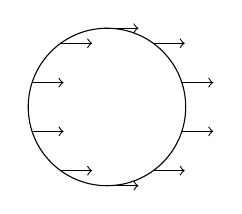
\begin{tikzpicture}
\draw (0,0) circle (1cm);
\foreach \rot in {36,72,...,360}{
\draw[->] ({sin(\rot)},{cos(\rot)}) -- +(.4,0);}
\end{tikzpicture}

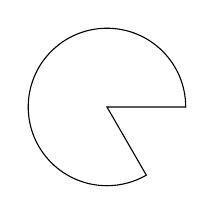
\begin{tikzpicture}
\draw (0,0) -- (1,0) arc (0:300:1cm) -- cycle;
\end{tikzpicture}

If the connection is metric compatible, the \ueig{metric is parallel transported}. This means parallel transport preserves properties like norm, orthogonality etc.

\subsection{Geodesics}
Two way of seeing it:
\begin{enumerate}
\item Parallel transports it's own tangent vector
\item Shortest distance between two points.
\end{enumerate}

\subsubsection{As a curve that parallel transports it's tangent vector}
Setting directional covariant derivative of $\od{x^\mu}{\lambda}$ to zero gives
\[ \frac{D}{d\lambda}\od{x^\mu}{\lambda} = \boxed{ \od[2]{x^\mu}{\lambda} + \Gamma^\mu_{\rho\sigma}\od{x^\rho}{\lambda}\od{x^\sigma}{\lambda} = 0 } \]
This is the \textbf{geodesic equation}. In flat space using Cartesian coordinates, this reduces to the equation of straight lines.

Actually this procedure constrains the parametrisation of the curve. In general a curve may be thought of as a geodesic if it parallel transports the \emph{unit} tangent vector. The in formula above the norm of the tangent vector was also forced to be constant. This constrains the parametrisation to be an \udef{affine parameter}, which is a parameter of the form
\[ \lambda = a\tau + b \]
with $\tau$ the arc length (i.e. proper time) and $a$ and $b$ constants.

Now say $\alpha$ is an arbitrary parametrisation and $v(\alpha) = \left|\od{x^\mu}{\alpha}\right|$ the norm of the tangent vector $\od{x^\mu}{\alpha}$. The unit tangent vector is then $v^{-1}\od{x^\mu}{\alpha}$. Requiring that this be parallel transported gives
\begin{align}
\frac{D}{d\alpha}\left(v^{-1}\od{x^\mu}{\alpha}\right) &= \od{x^\rho}{\alpha}\nabla_\rho\left[v^{-1}\od{x^\mu}{\alpha}\right] \\
&= \od{x^\rho}{\alpha} \left[\partial_\rho \left(v^{-1}\od{x^\mu}{\alpha}\right) + \Gamma^\mu_{\rho\sigma}v^{-1}\od{x^\sigma}{\alpha}\right] \\
&= \od{x^\rho}{\alpha} \left[\od{x^\mu}{\alpha}\partial_\rho v^{-1} + v^{-1}\partial_\rho \od{x^\mu}{\alpha} + \Gamma^\mu_{\rho\sigma}v^{-1}\od{x^\sigma}{\alpha}\right] = 0.
\end{align}
Multiplying both sides by $v$ gives
\[ 0 = \od{x^\mu}{\alpha}v\od{x^\rho}{\alpha}\partial_\rho v^{-1} + \od[2]{x^\mu}{\alpha} + \Gamma^\mu_{\rho\sigma}\od{x^\rho}{\alpha}\od{x^\sigma}{\alpha} \]
which is the geodesic equation derived above plus an extra term of the form $f(\alpha)\od{x^\mu}{\alpha}$, with
\begin{align}
f(\alpha) &= v \od{v^{-1}}{\alpha} \\
&= -v^{-1}\od{v}{\alpha} \\
&= - \left(\od[2]{\tau}{\alpha}\right)\left(\od{\tau}{\alpha}\right)^{-1}
\end{align}
using $v = \od{\tau}{\alpha}$, because the proper time is the arc length (TODO rephrase?). The factor $f(\alpha)$ is obviously zero for affine parameters.

For timelike paths we can write the geodesic equation in terms of the four-velocity $u^\mu = \od{x^\mu}{\tau}$:
\[ u^\lambda\nabla_\lambda u^\mu = 0 \]

For massive particles the four-momentum $p^\mu$ is $mu^\mu$, making this equivalent to
\[ p^\lambda\nabla_\lambda p^\mu = 0 \]

\subsubsection{As the shortest distance between two points}
\paragraph{For timelike paths.} Consider the proper time functional for a timelike path parametrised by $\lambda$:
\[ \tau_{AB} = \int \left(-g_{\mu\nu} \od{x^\mu}{\lambda}\od{x^\nu}{\lambda}\right)^{1/2} \diff{\lambda} \]
We want to find the stationary paths, with $\delta \tau = 0$. Computing the variation and setting $f = g_{\mu\nu} \od{x^\mu}{\lambda}\od{x^\nu}{\lambda}$ gives
\begin{align}
\delta \tau &= \int \delta\sqrt{-f}\diff{\lambda} \\
&= -\int \frac{1}{2}(-f)^{-1/2}\delta f \diff{\lambda}.
\end{align}

Now we can reparametrise the path, taking the proper time as the new parameter. This means the tangent vector is the four-velocity $u^\mu$, which fixes $f$
\[ f = g_{\mu\nu} \od{x^\mu}{\tau}\od{x^\nu}{\tau} = g_{\mu\nu}u^\mu u^\nu = -1, \]
so
\[ \delta \tau = - \frac{1}{2}\int\delta f \diff{\tau} \]

This means stationary paths of the proper time functional are also stationary paths of the simpler integral
\[ I = \frac{1}{2}\int f \diff{\tau} = \frac{1}{2}\int g_{\mu\nu} \od{x^\mu}{\tau}\od{x^\nu}{\tau} \]
and vice versa.

We can explicitly vary this integral with (TODO why)
\[ \begin{cases}
x^\mu \to x^\mu _ \delta x^\mu \\
g_{\mu\nu} \to g_{\mu\nu} + (\partial_\sigma g_{\mu\nu})\delta x^\sigma.
\end{cases} \]
Plugging this into the expression for $I$ and keeping only terms that are first order in $\delta x^\mu$, we get
\[ \delta I = \frac{1}{2}\int \left[\partial_\sigma g_{\mu\nu}\od{x^\mu}{\tau}\od{x^\nu}{\tau}\delta x^\sigma + g_{\mu\nu}\od{(\delta x^\mu)}{\tau}\od{x^\nu}{\tau} +g_{\mu\nu}\od{x^\mu}{\tau}\od{(\delta x^\nu)}{\tau}\right]\diff{\tau} \]
The last two terms can be integrated by parts; for example,
\begin{align}
\int \left[ g_{\mu\nu}\od{x^\mu}{\tau}\od{(\delta x^\nu)}{\tau} \right]\diff{\tau} &= \left. g_{\mu\nu}\od{x^\mu}{\tau}\delta x^\nu \right|_\text{at boundary} - \int \od{}{\tau}\left(g_{\mu\nu}\od{x^\mu}{\tau}\right)\delta x^\nu \diff{\tau} \\
&= - \int \left[g_{\mu\nu} \od[2]{x^\mu}{\tau} + \od{g_{\mu\nu}}{\tau}\od{x^\mu}{\tau}\right]\delta x^\nu \diff{\tau} \\
&= - \int \left[g_{\mu\nu} \od[2]{x^\mu}{\tau} + \partial_\sigma g_{\mu\nu}\od{x^\sigma}{\tau}\od{x^\mu}{\tau}\right]\delta x^\nu \diff{\tau}
\end{align}
where we have used that $\delta x^\nu$ vanishes at the boundary.

The total variation is then
\[ \delta I = - \int \left[g_{\mu\sigma}\od[2]{x^\mu}{\tau} + \frac{1}{2}\left(\partial_\mu g_{\nu\sigma} + \partial_\nu g_{\sigma\mu} - \partial_\sigma g_{\mu\nu}\right)\od{x^\mu}{\tau}\od{x^\nu}{\tau}\right]\delta x^\sigma \diff{\tau}. \]
Since we are searching for stationary points, we want $\delta I$ to vanish for any variation $\delta x^\sigma$. This implies that the expression inside the square brackets must vanish. Multiplying it with the inverse metric $g^{\rho\sigma}$ yields
\[ \od[2]{x^\rho}{\tau} + \frac{1}{2}g^{\rho\sigma}\left(\partial_\mu g_{\nu\sigma} + \partial_\nu g_{\sigma\mu} - \partial_\sigma g_{\mu\nu}\right)\od{x^\mu}{\tau}\od{x^\nu}{\tau} = 0 \]
Which is exactly the geodesic equation with the Christoffel symbols as the connection.

This procedure provides a convenient way to calculate the Christoffel symbols for a given metric: by explicitly varying the integral $I$ with the metric of interest plugged in.

\paragraph{Null geodesics.} The geodesic formula was found using a very specific parametrisation, which is not a problem because all regular curves can be arc parametrised. Unfortunately we also restricted ourselves to timelike paths, because for null paths $\tau = 0$.

Now the geodesic equation derived above is still perfectly valid, even if $\tau$ can no longer be considered a valid parameter. An affine parameter is now any parameter such that the geodesic equation is satisfied, but now there is no special one. They are all related by the fact that if $\lambda$ is an affine parameter, any parameter of the form $a\lambda + b$ is as well. 

It is often convenient to normalise the affine parameter $\lambda$ along a null geodesic such that
\[ p^\mu = \od{x^\mu}{\lambda} \]

\paragraph{Timelike geodesics are maxima.} Locally that is. We can see that this is true because any timelike path can be arbitrarily well approximated by a null curve.

\subsubsection{Exponential map}
TODO

Geodesically incomplete

Riemann normal coordinates

\subsection{Riemann curvature tensor}
We now want an object that embodies our idea of curvature. Seeing as we are going to define a new object to fit out intuition, we need to flesh it out a bit first. We begin by naming some properties of flat spacetime:
\begin{itemize}
\item Parallel transport around a closed loop leaves vectors unchanged;
\item Covariant derivatives of tensors commute;
\item Initially parallel geodesics remain parallel.
\end{itemize}
TODO motivation.
\udef{Riemann tensor $\tensor{\mathcal{R}}{^\rho_{\sigma\mu\nu}}$} is a $(1,3)$-tensor. It is antisymmetric in the last two indices.

\begin{align}
[\nabla_\mu,\nabla_\nu]V^\rho &= \nabla_\mu\nabla_\nu V^\rho - \nabla_\nu\nabla_\mu V^\rho \\
&= \left(\partial_\mu(\nabla_\nu V^\rho) - \Gamma^\lambda_{\mu\nu}\nabla_\lambda V^\rho + \Gamma^\rho_{\mu\sigma}\nabla_\nu V^\rho \right) - \left(\partial_\nu(\nabla_\mu V^\rho) - \Gamma^\lambda_{\nu\mu}\nabla_\lambda V^\rho + \Gamma^\rho_{\nu\sigma}\nabla_\mu V^\rho \right) \\
&= 2\left(\partial_{[\mu}(\nabla_{\nu]} V^\rho) - \Gamma^\lambda_{[\mu\nu]}\nabla_\lambda V^\rho + \Gamma^\rho_{[\mu|\sigma|}\nabla_{\nu]} V^\rho \right) \\
&= 2\left(\partial_{[\mu}\partial_{\nu]} V^\rho + \partial_{[\mu}(\Gamma^\rho_{\nu]\sigma} V^\sigma) - \Gamma^\lambda_{[\mu\nu]}\nabla_\lambda V^\rho + \Gamma^\rho_{[\mu|\sigma|}\partial_{\nu]} V^\sigma + \Gamma^\rho_{[\mu|\sigma|}\Gamma^\rho_{\nu]\sigma} V^\sigma \right) \\
&= \cancel{[\partial_{\mu}, \partial_{\nu}] V^\rho} + 2\left(\partial_{[\mu}(\Gamma^\rho_{\nu]\sigma} V^\sigma) - \Gamma^\lambda_{[\mu\nu]}\nabla_\lambda V^\rho + \Gamma^\rho_{[\mu|\sigma|}\partial_{\nu]} V^\sigma + \Gamma^\rho_{[\mu|\sigma|}\Gamma^\rho_{\nu]\sigma} V^\sigma \right) \\
&= 2\left(\partial_{[\mu}(\Gamma^\rho_{\nu]\sigma}) V^\sigma + \cancel{\partial_{[\mu}( V^\sigma)\Gamma^\rho_{\nu]\sigma}} - \Gamma^\lambda_{[\mu\nu]}\nabla_\lambda V^\rho + \cancel{\Gamma^\rho_{[\mu|\sigma|}\partial_{\nu]} V^\sigma} + \Gamma^\rho_{[\mu|\sigma|}\Gamma^\rho_{\nu]\sigma} V^\sigma \right) \\
&= 2\left(\partial_{[\mu}\Gamma^\rho_{\nu]\sigma} + \Gamma^\rho_{[\mu|\sigma|}\Gamma^\rho_{\nu]\sigma} \right) V^\sigma - 2\Gamma^\lambda_{[\mu\nu]}\nabla_\lambda V^\rho \\
&= \left(\partial_{\mu}\Gamma^\rho_{\nu\sigma} - \partial_{\nu}\Gamma^\rho_{\mu\sigma} + \Gamma^\rho_{\mu\sigma}\Gamma^\rho_{\nu\sigma} - \Gamma^\rho_{\nu\sigma}\Gamma^\rho_{\mu\sigma} \right) V^\sigma - \tensor{T}{^\lambda_{\mu\nu}}\nabla_\lambda V^\rho \\
&\equiv \tensor{\mathcal{R}}{^\rho_{\mu\nu\sigma}}V^\sigma - \tensor{T}{^\lambda_{\mu\nu}}\nabla_\lambda V^\rho
\end{align}

Where $[\;,\;]$ is the antisymmetrisation, $[\mu|\sigma|\nu]$ means that only $\mu$ and $\nu$ are antisymmetrised and $T$ is the torsion tensor. So the Riemann tensor is identified as
\[ \boxed{\tensor{\mathcal{R}}{^\rho_{\mu\nu\sigma}} \equiv \partial_{\mu}\Gamma^\rho_{\nu\sigma} - \partial_{\nu}\Gamma^\rho_{\mu\sigma} + \Gamma^\rho_{\mu\sigma}\Gamma^\rho_{\nu\sigma} - \Gamma^\rho_{\nu\sigma}\Gamma^\rho_{\mu\sigma}} \]

\subsubsection{Properties of the curvature tensor}
To investigate the properties of the Riemann tensor, the upper index is lowered
\[ \mathcal{R}_{\rho\sigma\mu\nu} = g_{\rho\lambda}\tensor{\mathcal{R}}{^\lambda_{\sigma\mu\nu}} \]
and an explicit expression is obtained in locally inertial coordinates. In locally inertial coordinates the metric and its first derivatives vanish, so the Christoffel symbols do as well, but not their derivatives.
\begin{align}
\mathcal{R}_{\hat{\rho}\hat{\sigma}\hat{\mu}\hat{\nu}} &= g_{\hat{\rho}\hat{\lambda}} \left(\partial_{\hat{\mu}}\Gamma^{\hat{\lambda}}_{\hat{\nu}\hat{\sigma}} - \partial_{\hat{\nu}}\Gamma^{\hat{\lambda}}_{\hat{\mu}\hat{\sigma}}\right) \\
&= \frac{1}{2}g_{\hat{\rho}\hat{\lambda}}g^{\hat{\lambda}\hat{\tau}}\left[\left(\partial_{\hat{\mu}}\partial_{\hat{\nu}}g_{\hat{\sigma}\hat{\tau}} + \partial_{\hat{\mu}}\partial_{\hat{\sigma}}g_{\hat{\tau}\hat{\nu}} - \partial_{\hat{\mu}}\partial_{\hat{\tau}}g_{\hat{\nu}\hat{\sigma}}\right) - \left(\partial_{\hat{\nu}}\partial_{\hat{\mu}}g_{\hat{\sigma}\hat{\tau}} + \partial_{\hat{\nu}}\partial_{\hat{\sigma}}g_{\hat{\tau}\hat{\mu}} - \partial_{\hat{\nu}}\partial_{\hat{\tau}}g_{\hat{\mu}\hat{\sigma}}\right)\right] \\
&= \frac{1}{2}\left[\partial_{\hat{\mu}}\partial_{\hat{\sigma}}g_{\hat{\rho}\hat{\nu}} - \partial_{\hat{\mu}}\partial_{\hat{\rho}}g_{\hat{\nu}\hat{\sigma}} - \partial_{\hat{\nu}}\partial_{\hat{\sigma}}g_{\hat{\rho}\hat{\mu}} + \partial_{\hat{\nu}}\partial_{\hat{\rho}}g_{\hat{\mu}\hat{\sigma}}\right]
\end{align}
This derivation was done in a special coordinate system, but all tensorial equations that follow from it must be true in any coordinate system. A few such equations are now listed:
\begin{enumerate}
\item The Riemann tensor is antisymmetric in its first two indices.
\[ \boxed{ \mathcal{R}_{\rho\sigma\mu\nu} = - \mathcal{R}_{\sigma\rho\mu\nu} } \]
\item The Riemann tensor is antisymmetric in its last two indices.
\[ \boxed{ \mathcal{R}_{\rho\sigma\mu\nu} = - \mathcal{R}_{\rho\sigma\nu\mu} } \]
\item The Riemann tensor is invariant under exchange of the first and last pair of indices.
\[ \boxed{ \mathcal{R}_{\rho\sigma\mu\nu} = \mathcal{R}_{\mu\nu\rho\sigma} } \]
\item Thus sum of cyclic permutations of the last three indices vanishes.
\[ \mathcal{R}_{\rho\sigma\mu\nu} + \mathcal{R}_{\rho\mu\nu\sigma} + \mathcal{R}_{\rho\nu\sigma\mu} = 0 \]
This is equivalent to the vanishing of the antisymmetric part of the last three indices.
\[ \boxed{  \mathcal{R}_{\rho[\sigma\mu\nu]} = 0 } \]
\end{enumerate}
\paragraph{Number of parameters.} TODO
\paragraph{Bianchi identity.} TODO
\[ \nabla_{[\lambda}\mathcal{R}_{\rho\sigma]\mu\nu} = 0 \]

\subsubsection{Derived quantities}
Tricks for decomposition: taking contractions and taking (anti)symmetric parts.

\paragraph{Ricci tensor.} This \udef{Ricci tensor} is defined as
\[ \mathcal{R}_{\mu\nu} \equiv \tensor{\mathcal{R}}{^\lambda_{\mu\lambda\nu}}. \]
The Ricci tensor associated with the Christoffel connection is automatically symmetric:
\begin{align}
\mathcal{R}_{\mu\nu} &= g^{\rho\lambda}\mathcal{R}_{\rho\mu\lambda\nu} = g^{\rho\lambda}\mathcal{R}_{\lambda\nu\rho\mu} = \tensor{\mathcal{R}}{^\rho_{\nu\rho\mu}} \\
&= \mathcal{R}_{\nu\mu}
\end{align}
The trace of the Ricci tensor is called the \udef{Ricci scalar} (or curvature scalar):
\[ R \equiv \tensor{\mathcal{R}}{^\mu_\mu} = g^{\mu\nu}\mathcal{R}_{\mu\nu} \]

Now a useful form of the Bianchi identity can be obtained by multiplying it by $3g^{\nu\sigma}g^{\mu\lambda}$:
\begin{align}
0 &= 3g^{\nu\sigma}g^{\mu\lambda}\nabla_{[\lambda}\mathcal{R}_{\rho\sigma]\mu\nu} \\
&= \frac{3g^{\nu\sigma}g^{\mu\lambda}}{6!}\left[\left(\nabla_{\lambda}\mathcal{R}_{\rho\sigma\mu\nu} + \nabla_{\rho}\mathcal{R}_{\sigma\lambda\mu\nu} + \nabla_{\sigma}\mathcal{R}_{\lambda\rho\mu\nu}\right) - \left(\nabla_{\lambda}\mathcal{R}_{\sigma\rho\mu\nu} + \nabla_{\rho}\mathcal{R}_{\lambda\sigma\mu\nu} + \nabla_{\sigma}\mathcal{R}_{\rho\lambda\mu\nu}\right)\right] \\
&= g^{\nu\sigma}g^{\mu\lambda}\left[\nabla_{\lambda}\mathcal{R}_{\rho\sigma\mu\nu} + \nabla_{\rho}\mathcal{R}_{\sigma\lambda\mu\nu} + \nabla_{\sigma}\mathcal{R}_{\lambda\rho\mu\nu}\right] \\
&= \nabla^\mu\mathcal{R}_{\rho\mu} - \nabla_\rho R + \nabla^\nu\mathcal{R}_{\rho\nu}
\end{align}
or
\[ \boxed{\nabla^\mu\mathcal{R}_{\rho\mu} = \frac{1}{2}\nabla_\rho R.} \]


\paragraph{Weyl tensor.} TODO Why. In $n$ dimensions the \udef{Weyl tensor} is given by
\[ C_{\rho\sigma\mu\nu} \equiv \mathcal{R}_{\rho\sigma\mu\nu} - \frac{2}{n-2}\left(g{\rho[\mu}\mathcal{R}_{\nu]\sigma} - g{\sigma[\mu}\mathcal{R}_{\nu]\rho}\right) + \frac{2}{(n-1)(n-2)}g{\rho[\mu}\mathcal{R}_{\nu]\sigma} \]
TODO properties.

\paragraph{Einstein tensor.} The \udef{Einstein tensor} is defined as
\[ G_{\mu\nu} \equiv \mathcal{R}_{\mu\nu} - \frac{1}{2}Rg_{\mu\nu}. \]
Now the Bianchi identity reduces to
\[ \boxed{\nabla^{\mu}G_{\mu\nu} = 0} \]


\section{Isometries}
\subsection{About isometries}
TODO post geometry.
\[ g'_{\mu\nu}(y) = g_{\mu\nu}(y) \]

Symmetries of arbitrary tensor fields.
\subsection{Lie derivatives}
In general $g_{\mu\nu}(x_p)$ is different from $g_{\mu\nu}(x_q)$. Are there directions we can move in on the manifold so that the metric (or any other function on the manifold) doesn't change.
So we want
\[ g_{\mu\nu}(\tilde{x}) = \pd{x^\rho}{\tilde{x}{^\mu}}\pd{x^\sigma}{\tilde{x}{^\nu}}g_{\rho\sigma}(x) \]
to equal the original metric.

We consider an infinitessimal transformation:
\[ \tilde{x}^\mu = x^\mu+\epsilon V^\mu \]
\[ \delta y^\mu = \pd{y^\mu}{x^\nu}\delta x^\nu \]

\subsubsection{Lie derivative on a scalar}
We are comparing
\[  \begin{cases}
\phi(\tilde{x}) = \phi(x + \epsilon V) = \phi(x) + \epsilon V^\mu\partial_\mu \phi(x) + \mathcal{O}(\epsilon^2) \\
\tilde{\phi}(\tilde{x}) = \phi(x)
\end{cases}\]

\begin{align}
L_V\phi &\equiv \lim_{\epsilon\to 0}\frac{\phi(\tilde{x}) - \tilde{\phi}(\tilde{x})}{\epsilon} \\
&= \lim_{\epsilon\to 0}\frac{\phi(x+\epsilon V^\mu)-\phi(x)}{\epsilon} \\
&= \lim_{\epsilon\to 0}\frac{\cancel{\phi(x)}+\epsilon V^\mu\partial_\mu\phi(x)+\mathcal{O}(\epsilon^2)-\cancel{\phi(x)}}{\epsilon} \\
&= V^\mu\partial_\mu\phi(x)
\end{align}

Ordinary directional derivative.

In general:
\[ L_V: (p,q) \text{forms} \to (p,q) \text{forms} \]

\subsubsection{Lie derivative of a vector field}
Again we define
\[ L_VW^\mu \equiv \lim_{\epsilon\to 0}\frac{W^\mu(\tilde{x}) - \tilde{W^\mu}(\tilde{x})}{\epsilon} \]
Again we are comparing two quantities
\begin{align}
W(\tilde{x}) &= W(x + \epsilon V) = W(x) + \epsilon V^\mu\partial_\mu W(x) + \mathcal{O}(\epsilon^2) \\
\tilde{W}(\tilde{x}) &= \pd{\tilde{x}^\mu}{x^\nu}W^\nu (x) \\
&= \pd{(x^\mu+\epsilon V^\mu)}{x^\nu}W^\nu (x) \\
&= \left(\delta^\mu_\nu+\epsilon \pd{V^\mu}{x^\nu}\right)W^\nu (x) \\
&= W^\mu (x)+\epsilon W^\nu (x)\partial_\nu V^\mu
\end{align}

Putting everything together, we get
\[ L_V W^\mu = V^\nu\partial_\nu W^\mu - W^\nu \partial_\nu V^\mu \]

Normal derivative not covariant, but here same as covariant derivative (extra bits cancel).

Not defined with respect to any particular metric.

Some properties:
\begin{itemize}
\item Partial derivatives can be replaced by covariant ones.
\item The Lie derivative is antisymmetric in $V$ and $W$ and defines a commutator
\[ [V,W]^\mu \equiv L_VW^\mu = - L_WV^\mu \]
This satisfies the Jacobi identity 
\[ [V,[W,X]]^\mu + [X,[V,W]]^\mu + [W,[X,V]]^\mu \]
and thus is a Lie bracket.  The Jacobi identity is equivalent to
\[ L_V[W,X]^\mu = [L_VW,X]^\mu + [W,L_VX]^\mu \]
\end{itemize}


\subsubsection{Lie derivative of other tensor fields}
The definitions above are readily generalised
\[ \tilde{x}^\mu(x) = x^\mu +\epsilon V^\mu(x) \]
\[ L_VT = \lim_{\epsilon\to 0} \frac{T(\tilde{x})-\tilde{T}(\tilde{x})}{\epsilon} \]
where we need
\[ \pd{\tilde{x}^\mu}{x^\rho} = \delta^\mu_\rho + \epsilon \partial_\rho V^\mu + \mathcal{O}(\epsilon^2) \qquad \text{and}\qquad \pd{x^\mu}{\tilde{x}{^\rho}} = \delta^\mu_\rho - \epsilon \partial_\rho V^\mu + \mathcal{O}(\epsilon^2) \]

Again partial derivatives can be replaced by covariant derivatives. We illustrate with a $(0,2)$-tensor $T_{\mu\nu}$.
\[ \begin{cases}
T_{\mu\nu}(\tilde{x}) = T_{\mu\nu}(x) + \epsilon V^\rho\partial_\rho T_{\mu\nu}+ \mathcal{O}(\epsilon^2) \\
\tilde{T}_{\mu\nu}(\tilde{x}) = \pd{x^\mu}{\tilde{x}{^\mu}}\pd{x^\nu}{\tilde{x}{^\nu}}T_{\mu\nu} = T_{\mu\nu} - \epsilon\partial_\mu V^\rho T_{\rho\nu}(x) - \epsilon\partial_\nu V^\sigma T_{\mu\sigma} + \mathcal{O}(\epsilon^2)
\end{cases} \]
Filling this in gives
\begin{align}
L_V T_{\mu\nu} &= \lim_{\epsilon\to 0} \frac{T_{\mu\nu}(\tilde{x})-\tilde{T}_{\mu\nu}(\tilde{x})}{\epsilon} \\
&= \lim_{\epsilon\to 0} \frac{\cancel{T_{\mu\nu}(x)}+\epsilon V^\rho\partial_\rho T_{\mu\nu}+ \mathcal{O}(\epsilon^2)-\cancel{T_{\mu\nu}}+\epsilon T_{\rho\nu} \partial_\mu V^\rho +\epsilon T_{\mu\sigma} \partial_\nu V^\sigma + \mathcal{O}(\epsilon^2)}{\epsilon} \\
&= V^\rho\partial_\rho T_{\mu\nu} + T_{\rho\nu} \partial_\mu V^\rho + T_{\mu\rho} \partial_\nu V^\rho \\
&= V^\rho \left(\nabla_\rho T + \Gamma^\lambda_{\rho \mu}T_{\lambda \nu} + \Gamma^\lambda_{\rho \nu}T_{\mu \lambda} \right) + T_{\rho\nu} \left(\nabla_\mu V^\rho - \Gamma^\rho_{\mu\lambda}V^\lambda\right) + T_{\mu\rho} \left(\nabla_\nu V^\rho - \Gamma^\rho_{\nu\lambda}V^\lambda\right) \\
&= V^\rho\nabla_\rho T + T_{\rho\nu}\nabla_\mu V^\rho + T_{\mu\rho}\nabla_\nu V^\rho + \left(\Gamma^\lambda_{\rho \mu}V^\rho T_{\lambda \nu} - \Gamma^\rho_{\mu\lambda}V^\lambda T_{\rho\nu}\right) + \left(\Gamma^\lambda_{\rho \nu}V^\rho T_{\mu \lambda} - \Gamma^\rho_{\nu\lambda}V^\lambda T_{\mu\rho}\right) \\
&= V^\rho\nabla_\rho T + T_{\rho\nu}\nabla_\mu V^\rho + T_{\mu\rho}\nabla_\nu V^\rho
\end{align}

Isometries from an algebra
\[ \left[L_V,L_W\right] = L_{[V,W]} \]
Enough to verify scalars and vectors.

\subsubsection{Lie derivative of tensor densities}
TODO

\subsection{Killing vectors}
The Lie derivative of the metric tensor. This is $(0,2)$-tensor, so the formula is the one given above.
Due to metric compatibility, the first term is zero
\begin{align}
L_V g_{\mu\nu} &= V^\rho\nabla_\rho g_{\mu\nu} + g_{\lambda\nu}\nabla_\mu V^\lambda + g_{\mu\lambda}\nabla_\nu V^\lambda \\
&= g_{\lambda\nu}\nabla_\mu V^\lambda + g_{\mu\lambda}\nabla_\nu V^\lambda \\
&= \nabla_\mu V_\nu + \nabla_\nu V_\nu \\
\end{align}

An infinitesimal coordinate transformation is a symmetry of the metric if $L_V g_{\mu\nu} = 0$, which is equivalent to requiring $V$ to satisfy the equations
\[ \nabla_\mu V_\nu + \nabla_\nu V_\nu = 0 = \nabla_{(\mu} V_{\nu)}. \]
Such vectors are called \udef{Killing vectors}. These equations are equivalent to
\[ \nabla_\mu V_\nu = \nabla_{[\mu}V_{\nu]} \]


Properties:
\begin{enumerate}
\item Killing vectors form a Lie algebra. If $V$ and $W$ are Killing vectors, i.e. $L_Vg_{\mu\nu} = L_Wg_{\mu\nu} = 0$, then $[V,W]$ is a Killing vector because
\[ L_{[V,W]}g_{\mu\nu} = L_VL_Wg_{\mu\nu} - L_WL_V g_{\mu\nu} = 0  \]
\item If all the components of the metric are independent of a particular coordinate, say $y$
\[ \partial_y g_{\mu\nu} \qquad \forall \mu,\nu \]
Then $V=\partial_y$ is a Killing vector. A coordinate system in which a Killing vector is a partial derivative is said to be \textit{adapted} to the Killing vector (or isometry) in question. TODO derive Killing equations from this.
\item Two Killing vectors commute if and only if there is a coordinate system that is adapted to both of them.
\end{enumerate}

You can use the equations in 2 ways:
\begin{itemize}
\item Impose symmetries on the metric.
\item Find the Killing vectors for a given metric, which gives the symmetries
\end{itemize}

\begin{example}
Algebra of Killing vectors in Minkowski and two-sphere.
\end{example}

\subsection{Conserved quantities}
\subsubsection{Conserved charges along geodesics}
Let $K^\mu$ be a Killing vector field and $x^\mu(\tau)$ a geodesic with four-velocity $x^\mu$. Then the quantity
\[ Q_K = K_\mu u^\mu \]
is constant along the geodesic. Indeed,
\begin{align}
\od{}{\tau}Q_K = \od{K_\mu u^\mu}{\tau} &= u^\mu \od{K_\mu}{\tau} + K_\mu \od{}{\tau}u^\mu \\
&= u^\mu u^\nu \nabla_\nu K_\mu + 0\\
&= \frac{1}{2}\left(\nabla_\nu K_\mu + \nabla_\mu K_\nu\right)u^\mu u^\nu = 0
\end{align}
where the last equality is due to the Killing equations.

\subsubsection{Conserved currents from the energy-momentum tensor}
Let $K^\mu$ be a Killing vector field and $T^{\mu\nu}$ the covariantly conserved symmetric energy-momentum tensor ($\nabla_\mu T^{\mu\nu} = 0$). Then the current
\[ J_K^\mu = T^{\mu\nu}K_\nu \]
is covariantly conserved. Indeed,
\begin{align}
\nabla_\mu J^\mu_K &= (\nabla_\mu T^{\mu\nu})K_\nu + T^{\mu\nu} \nabla_\mu K_\nu \\
&= 0 + \frac{1}{2}T^{\mu\nu}\left(\nabla_\mu K_\nu + \nabla_\nu K_\mu\right) = 0
\end{align}

\subsubsection{Komar currents}
The Einstein tensor is symmetric and conserved (from the Bianchi identity), so we have the conserved current
\[ J^\mu_1 = \tensor{G}{^\mu_\nu}K^\nu =  \]

\subsection{Killing tensors}

\subsubsection{Killing(-Stäckel) tensors}
A \udef{Killing tensor $K_{\beta_1\ldots\beta_n}$} is a totally symmetric tensor satisfying
\[ \nabla_{(\alpha}K_{\beta_1\ldots\beta_n)} = 0. \]

The charge
\[ Q_K = K_{\beta_1\ldots\beta_n}u^{\beta_1}\ldots u^{\beta_n} \]
is constant along the geodesic.

\subsubsection{Killing-Yano tensors}
A \udef{Killing-Yano tensor $Y_{\beta_1\ldots\beta_n}$} is a totally anti-symmetric tensor satisfying
\[ \nabla_{(\alpha} Y_{\beta_1)\ldots\beta_n} = 0 \qquad \text{or, equivalenty} \qquad \nabla_\alpha Y_{\beta_1\ldots\beta_n} = \nabla_{[\alpha}Y_{\beta_1\ldots\beta_n]} \]

The tensorial charges
\[ Z_{\beta_1\ldots\beta_{n-1}} = u^\beta Y_{\beta\beta_1\ldots\beta_{n-1}} \]
are conserved along geodesics.


\subsubsection{Symmetries and conserved charges (Komar integrals)}
\subsubsection{Conservation laws}
Conservation laws
\begin{itemize}
\item for geodesics
\item for spacetime
\end{itemize}

\[ Q = V^\mu \od{x^\nu}{\tau}g_{\mu\nu} \]
$\od{}{\tau}Q$ if $V$ is Killing and $\dot{x}^\mu$ is a geodesic.
\begin{align}
\od{}{\tau}Q = \od{}{\tau}\left(V_\mu\dot{x}^\mu\right) &= \left(\frac{DV_\mu}{D\tau}\right)\dot{x}^\mu + V_\mu \frac{D\dot{x}^\mu}{\tau} \\
&= \underbrace{\dot{x}^\rho D_\rho V_\mu \dot{x}^\mu}_{=0 \text{because Killing}} + \underbrace{V_\mu \frac{D\dot{x}^\mu}{D\tau}}_{=0 \text{geodesic}}
\end{align}

\subsection{Maximally symmetric spaces}
In D=4, maximally 10 symmetries. Minkowski maximally symmetric, but not uniquely so.
(Depends on number of killing vectors (which also form an algebra and can commute or not))

\[ K^\mu(x) \text{Killing} \quad \Leftrightarrow \quad D_{[\mu}K_{\nu]} = 0 \]
\[ K_\mu(x) = K_\mu(x^*) + \partial_\nu K_\mu(x^*)(x^\nu-x^{\nu*}) + \frac{1}{2}\partial_\rho\partial_\nu K_\mu(x^*)(x^\nu-x^{\nu *}(x^\rho - x^{\rho*}) + \ldots \]

\[ D_\mu K_\nu = \partial_\mu K_\nu - \Gamma^\rho_{\mu\nu}K_\rho \]
\[ \partial_\nu K_\mu(x^*) = D_\nu K_\mu(x^*) + \Gamma_{\nu\mu}^{\;\;\rho}K_\rho(x^*) \]
With
\[ D_\nu K_\mu(x^*) = \underbrace{\cancel{D_{(\nu}K_{\mu)}}}_{0 \text{because Killing}} + D_{[\nu}K_{\mu]}(x^*) \]
So
\[ \frac{D(D-1)}{2} \qquad \text{for} D=4 \quad \Rightarrow \quad 6 \text{coeff.} \]

Maximally symmetric:
\begin{itemize}
\item Minkowski: 4 translations, 6 Lorentz ($\Lambda = 0$)
\[ [P_\mu, P_\nu] = 0, \qquad [M_{\mu\nu}, P_\rho] = 2 \eta_{\rho[\mu}P_{\nu]}, \qquad [M_{\mu\nu}, M^{\rho\sigma}] = 4 \delta_{[\mu}^{\;\;[\rho}M_{\nu]}^{\;\;\sigma]} \]
\[M^{\mu\nu} = x^\mu\partial^\nu - x^\nu\partial^\mu \qquad G=\R^4 \rtimes \SO(1,3)\]
\item de Sitter $G = \SO(1,4)$ ($\Lambda>0$)
\item Anti-de Sitter $G=\SO(2,3)$
\end{itemize}
On a side note
\[ dS_4 \equiv \frac{\SO(1,4)}{\SO(1,3)} \qquad AdS_4 \equiv \frac{\SO(2,3)}{\SO(1,3)} \]
Confer:
\[ S^p = \frac{\SO(p+1)}{\SO(p)} \]

riemann normal coordinates + freely falling frames

\section{Conformal transformations}
\subsection{Conformal Killing vectors}
\[ L_C g_{\mu\nu} = \nabla_\mu C_\nu + \nabla_\nu C_\mu = 2\omega(x)g_{\mu\nu} \]

A Killing vector for a metric is at least a conformal Killing vector for any conformally rescaled metric.

\subsubsection{Conserved charges along null geodesics}
\[ Q_C = C_\mu u^\mu \]
\subsubsection{Conserved currents from the energy-momentum tensor}
energy-momentum tensor is traceless
\[ J_C^\mu = T^{\mu\nu}C_\nu \]

\subsection{Conformal Killing(-Yano) tensors}
